\section{Durchführung}
\label{sec:Durchführung}
In diesem Versuch werden die gemessene Fließgeschwindigkeit und das Strömungsprofil als Funktion der realen Strömungsgeschwindigkeit und des Dopplerwinkels untersucht. 
Es werden drei verschiedene Leitungen mit Innenradien von $7$, $10$ und $\qty{16}{\milli\metre}$ verwendet. 

\subsection{Vorbereitungsaufgaben}
\label{subsec:Vorbereitung}
Zur Vorbereitung des Versuches sollen die Dopplerwinkel $\alpha_i$ zu verschiedenen Prismenwinkeln $\theta_i$ berechnet werden. Dazu werden der enstprechende Winkel
$\theta$, die Ausbreitungsgeschwindigkeit $c_\text{P} = \qty{2700}{\metre\per\second}$ des Schalles im Prisma und die Ausbreitungsgeschwindigkeit
$c_\text{L} = \qty{1800}{\metre\per\second}$ in der Dopplerphantomflüssigkeit in \autoref{eqn:alpha} eingesetzt, wodurch die Werte
\begin{align*}
    \theta &= \qty{15}{\degree}: \qquad \alpha = \qty{80.04}{\degree} \\
    \theta &= \qty{30}{\degree}: \qquad \alpha = \qty{70.47}{\degree} \\
    \theta &= \qty{45}{\degree}: \qquad \alpha = \qty{60.00}{\degree} \\
    (\theta &= \qty{60}{\degree}: \qquad \alpha = \qty{54.72}{\degree}) \\
\end{align*} 
berechnet werden können.

\subsection{Versuchsaufbau}
\label{subsec:Aufbau}
Zur Durchführung des Versuches wird ein Ultraschall-Doppler-Generator verwendet. Dieser wird im Impuls-Echo-Verfahren mit einer $\qty{2}{\mega\hertz}$ Sonde betrieben.
Untersucht wird ein Rohrkreislauf, in welchem drei Rohre mit unterschiedlichen Durchmessern und zugehörige Prismen verbaut sind. Die Prismen sind an den jeweiligen
Rohrduchmesser angepasst und verfügen über je drei Flächen mit verschiedenem Dopplerwinkel, wobei alle Flächen den gleichen Abstand zur Probe (Flüssigkeit) garantieren.  
Der Aufbau der Prismen ist \autoref{fig:Prisma} zu entnehmen. Es wird eine aus Wasser, Glycerin und
Glasperlen bestehende Dopplerphantomflüssigkeit verwendet, dessen Viskosität $\eta$ und akustischen Eigenschaften auf den Versuchsaufbau abgestimmt sind.
Der Wasserkreislauf wird durch eine Zentrifugalpumpe angetrieben, welche die Durchflussmengen von $0$ bis $\qty{10}{\liter}$ liefert.
Die Signale des Echoskops werden an einen Rechner übertragen, an welchem sie mithilfe des Programms \textit{FlowView} ausgewertet werden können.

\begin{figure}
    \centering
    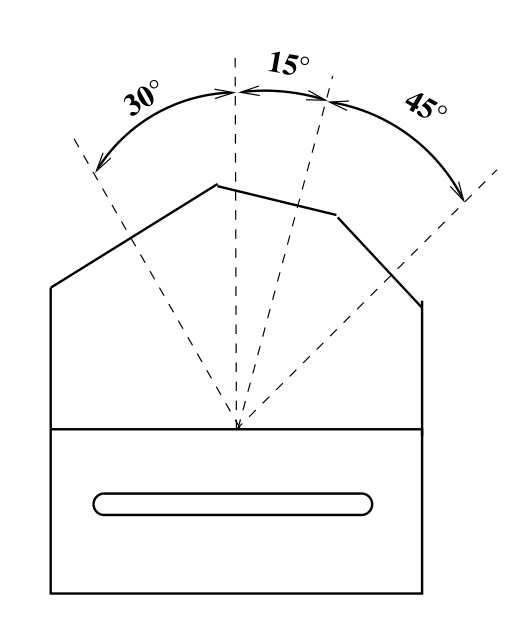
\includegraphics[width=.2\textwidth]{content/Prisma.png}
    \caption{Skizze des Prismas.}
    \label{fig:Prisma}
\end{figure}  

\subsection{Messaufgaben}
\label{subsec:Messaufgaben}
Zuerst wird die Strömungsgeschwindigkeit in Abhängigkeit zum Dopplerwinkel untersucht. Dazu muss der Regler \textit{SAMPLE VOLUME} des Ultraschall-Echoskops auf \textit{LARGE}
gestellt werden. An der Zentrifugalpumpe wird eine Drehzahl (Fließgeschwindigkeit) eingestellt. An den drei Flächen der Prismen werden Messwerte zur Bestimmung der 
Frequenzverschiebung $\symup{\Delta}\nu$ genommen, welche sich aus der Differenz der Anzeigen $f_\text{mean}$ und $f_\text{max}$ berechnet. Dieses Vorgehen wird für alle 
drei Rohrduchmesser mit je fünf Fließgeschwindigkeiten wiederholt. Aus den erhaltenen Werten lässt sich die Strömungsgeschwindigkeit zu den verschiedenen Dopplerwinkeln
berechnen. Anschließend wird der Ausdruck $\symup{\Delta}\nu \mathbin{/} \symup{cos}(\alpha)$ als Funktion der Strömungsgeschwindigkeit in einem Diagramm aufgetragen.
 
Im zweiten Teil des Versuches wird das Strömungsprofil der Dopplerflüssigkeit vermessen. Es wird lediglich der mittlere Schlauch mit einem Durchmesser von 
$\qty{15}{\milli\metre}$ unter einem Einstrahlwinkel von $\theta = \qty{15}{\degree}$ verwendet. \textit{SAMPLE VOLUME} muss dabei auf \textit{SMALL} gestellt werden,
um die Messtiefe regulieren zu können. Diese ist in $\unit{\micro\second}$ angegeben und kann unter \textit{DEPTH} eingestellt werden. In Acryl (Material des Prismas) 
entsprechen $\qty{4}{\micro\second}$ $\qty{10}{\milli\metre}$, in der Dopplerflüssigkeit entspricht dies $\qty{6}{\milli\metre}$. Die Messung beginnt in einer Tiefe
von $\qty{12}{\micro\second}$ und endet mit einer Schrittweite von $\qty{0.5}{\micro\second}$ bei $\qty{19.5}{\micro\second}$. Zu jedem Messpunkt werden die 
Intensität $I$, die Frequenzverschiebung $\symup{\Delta}\nu$ und die momentane Geschwindigkeit $v$ notiert. 
Dieses Messprogramm wird bei einer Pumpleistung von $\qty{45}{\percent}$ und $\qty{70}{\percent}$ der Maximalleistung durchgeführt.
Aus den Messwerten lässt sich die Struktur des Strömungsprofils ermitteln, indem Intensität und Geschwindigkeit gegen die Messtiefe aufgetragen werden.
